
We define a set of \emph{local} formulae. A formula is local if its groundings 
relate any number of observed ground atoms to exactly one hidden ground atom.  
For example, a grounding of the local formula \[lemma(p,+l_1) \wedge 
lemma(a,+l_2) \Rightarrow hasRole(p,a)\]
can be seen in the Markov Network of Figure \ref{fig:local2}. It connects a 
hidden \emph{hasRole} ground atom to two observed \emph{lemma} ground atoms.  
Note that the ``+'' prefix for variables indicates that there is a different 
weight for each possible pair of lemmas $(l_1,l_2)$.

\begin{figure}
\begin{center}
    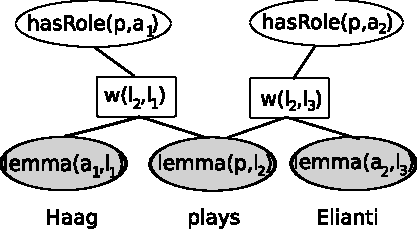
\includegraphics[scale=.70]{LocalFormula2}
\end{center}
\caption{Factor graph for the local formula in section \ref{sec:local}.}
\label{fig:local2}
\end{figure}

For predicates we defined local formulae that aimed to reproduce the standard 
features used in previous work~\citep{xue04calibrating}.  This also required us 
to develop dependency-based versions of the constituent-based features such as 
the syntactic path between predicate and argument, as proposed by 
\citet{xue04calibrating}. Table \ref{tbl:difs} shows the main differences of the 
models for each language. The features formulae corresponds to the FEAT column 
provided in the corpus. The presence of these formulae is determined by the 
availability of this information on the corpus. The sense formula corresponds to 
the formulae to model the sense of an SRL predicate. The use of the formulae is 
defined if the corpus labels the senses of the predicates. Finally, the formulae 
for the siblings of the arguments looks at the head of the children of the 
predicate and correlates them with an potential argument. These formulae show to 
provide an improvement for japanese during development. 

\begin{table}
\begin{center}
\small
\begin{tabular}{|l|c|c|c|}\hline
Formulae        & Features   & Sense  & Children  \\
                &                     & predicate   \\\hline\hline
Catalan         &   Yes      &  Yes   &  No  \\
Chinese         &   No       &  Yes   &  No  \\
Czech           &   Yes      &  No    &  No  \\
English         &   No       &  Yes   &  No  \\
German          &   Yes      &  Yes   &  No  \\
Japanese        &   Yes      &  No    &  Yes \\
Spanish         &   Yes      &  Yes   &  No  \\
\hline
\end{tabular}
\caption{Difference of formulae between the languages.}
\label{tbl:results}
\normalsize
\end{center}
\end{table}

Instead of describing the local feature set in more detail we refer the reader 
to our MLN model files.  
\footnote{\url{http://thebeast.googlecode.com/svn/mlns/conll09}} They can be 
used both as a reference and as input to our Markov Logic 
Engine\footnote{\url{http://thebeast.googlecode.com}}, and thus allow the reader 
to easily reproduce our results. We believe that this is another advantage of 
explicitly separating model and algorithms by using first order probabilistic 
logic languages.

